\documentclass{beamer}

\usepackage[utf8]{inputenc}
\usepackage[T1]{fontenc}
\usepackage[francais]{babel}
\usetheme{Warsaw}

\title{Stage de 5\ieme année}
\subtitle{Éco-conception de logiciel}
\author{Guillaume Delamare}
\institute{EMN - Équipe ASCOLA}
\date{\today}

\AtBeginSection[]
{
  \begin{frame}<beamer>
    \frametitle{Plan}
    \tableofcontents[currentsection, hideallsubsections]
  \end{frame}
}

\begin{document}
    \begin{frame}
	\titlepage
    \end{frame}

    \section*{Introduction}
	\begin{frame}
	    \frametitle{Plan}
	    \tableofcontents[hideallsubsections]{}
	\end{frame}
	
    \section{Présentation du sujet de stage}
	\begin{frame}{Contexte}
	    \begin{itemize}
		\item Travaux GreenIT de l'équipe ASCOLA
		\item
	    \end{itemize}
	\end{frame}
    	\begin{frame}{Sujet}
	    \begin{itemize}
		\item Forte augmentation des équipements informatique de part le monde
		\item La consommation d'énergie des système d'information un enjeu pour le future
		\item Plusieurs travaux sur la consommation du matériel
		\item Peu de travaux sur la consommation de la couche logicielle
	    \end{itemize}
	\end{frame}
	\begin{frame}{Objectifs}
	    Émettre des recommandations pour rendre moins énergivore les logiciels
	    \begin{block}{Pour cela il faut :}
	    \begin{itemize}
		\item Identifier les travaux réaliser dans le domaine
		\item Identifier des méthodes permettant de vérifier l'efficacité de ces recommandations
		\item Faire des propositions et les expérimenter
	    \end{itemize}
	    \end{block}
	\end{frame}
		
    \section{Mesure de la consommation}
	\begin{frame}{Outils de mesure de la consommation}
	    \begin{block}{Liste des outils testés}
		\begin{itemize}
		    \item pTop
		    \item Energy Checker
		    \item ClassMexer
		    \item JouleMeter
		    \item PowerAPI
		\end{itemize}
	    \end{block}	
	\end{frame}
	
	
    \section{Bonnes pratiques de programmation}
	\begin{frame}{Exemple de bonnes pratiques}
    	    \begin{block}{En java}
		Utiliser un StringBuffer pour manipuler une chaine de caractère plutot qu'un String.
	    \end{block}
    	    \begin{block}{En C}
		Faire attention à l'ordre des déclarations dans une structure.
	    \end{block}
	\end{frame}
	
    \section{Architecture logicielle}
	\begin{frame}{Modularité du code}
	    \begin{block}{OSGi}
		\begin{itemize}
		    \item Une spécification écrite par l'OSGi Alliance
		    \item Différentes inplémentations
		    \item Un système perméttant de construire des applications modulaires
		\end{itemize}
	    \end{block}
	\end{frame}
	\begin{frame}{Modularité du code}
	    \begin{center}
		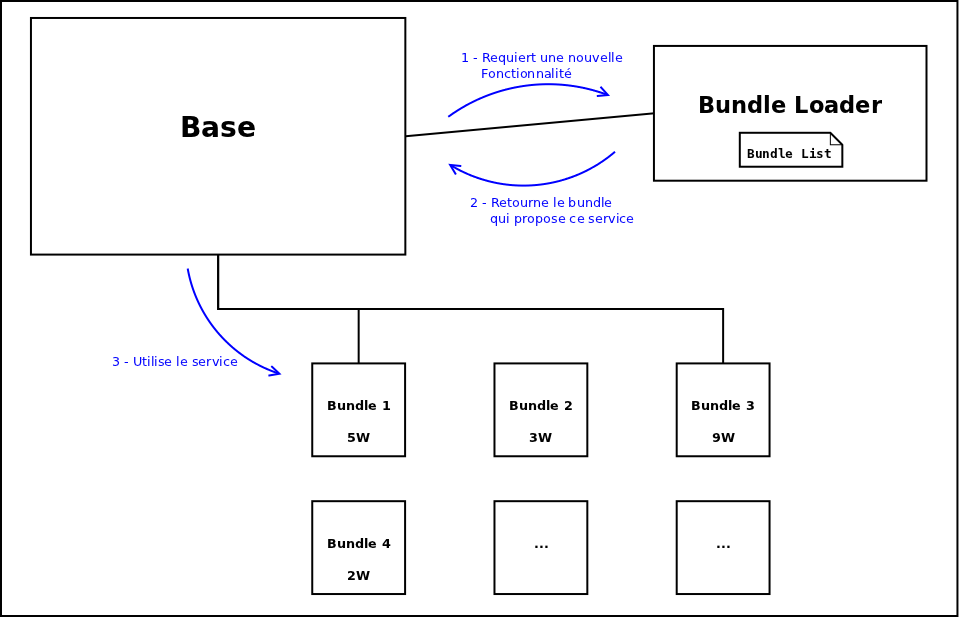
\includegraphics[width=200px]{../../Figures/OSGi/EcoPattern_General_Figure.png}
	    \end{center}
	\end{frame}
	
    \section{Conclusion}
	\begin{frame}{Conclusion}
	    	
	\end{frame}

    \section*{Questions}
	\begin{frame}{Questions}
	    \begin{columns}[c]
		\begin{column}{5cm}
		    Avez vous des questions ?
		\end{column}
    		\begin{column}{5cm}
    		    \begin{figure}
			%\includegraphics[width=6cm]{diagramme/}
		    \end{figure}
		\end{column}
	    \end{columns}
	\end{frame}
\end{document}
